\documentclass[12pt]{article}

\usepackage[utf8]{inputenc}
\usepackage[russian]{babel}
\usepackage{graphicx}
\usepackage{indentfirst}
\usepackage{booktabs}
\usepackage{amsmath}
\usepackage{tabto}


\graphicspath{{pic/}}

\begin{document}

%\begin{center}
%	\textbf{ФЕДЕРАЛЬНОЕ ГОСУДАРСТВЕННОЕ АВТОНОМНОЕ ОБРАЗОВАТЕЛЬНОЕ УЧРЕЖДЕНИЕ ВЫСШЕГО ОБРАЗОВАНИЯ}\\
%	 \\

%	\textbf{САНКТ-ПЕТЕРБУРГСКИЙ НАЦИОНАЛЬНЫЙ ИССЛЕДОВАТЕЛЬСКИЙ УНИВЕРСИТЕТ ИНФОРМАЦИОННЫХ ТЕХНОЛОГИЙ, МЕХАНИКИ И ОПТИКИ}\\

%\end{center}

\begin{center}
	\LARGE 
	\textbf{Лабораторная работа 2}\\
	Датчики случайных чисел. Построение гистограмм
	\\[3\baselineskip]
\end{center}

\begin{flushright}
	\large
	Выполнил:\\
	студент гр. P4106\\
	Игнашов Иван Максимович\\
	Вариант 8\\
\end{flushright}

\newpage

 \section*{1. Цель работы}
Изучение алгоритмов получения на ЭВМ чисел с заданным законом
распределения и построения гистограмм

\subsection*{Порядок работы:}
\begin{enumerate}
	\item Выбрать закон распределения верятностей. В соответствии с вариантом: Эрланговский закон с параметрами $k=3, \lambda=4$
	\item Вывести соотношение, позволяющее из чисел, сформированных базовым
датчиком, получить числа с заданным законом распределения
	\item Написать программу, реализующую датчик случайных чисел с заданным
законом распределения
	\item Написать программу построения гистограммы выборки, сформированной
созданным датчиком с учетом параметров
	\item При помощи программы построения гистограмм заполнить таблицу распределения элементов выборки по квантам гистограммы
	\item На основании таблицы построить гистограмму распределения сформированной выборки
	\item Построить график зависимости оценок математического ожидания и
дисперсии от объема выборки
\end{enumerate}

\newpage
 \section*{2. Формула и график моделируемого закона распределения}%
Плотность вероятности распределения по закону Эрланга:\\
$f(x; k, \lambda) = \frac{\lambda^kx^{k - 1}e^{-\lambda x}}{(k-1)!} $ для $ x,\lambda \geq 0$\\ \\
$f(x; 3, 4) = \frac{64x^{2}e^{-4 x}}{2} = 32x^2e^{-4 x} $ для $ x \geq 0$

 \begin{figure}[!h]
	\centering
	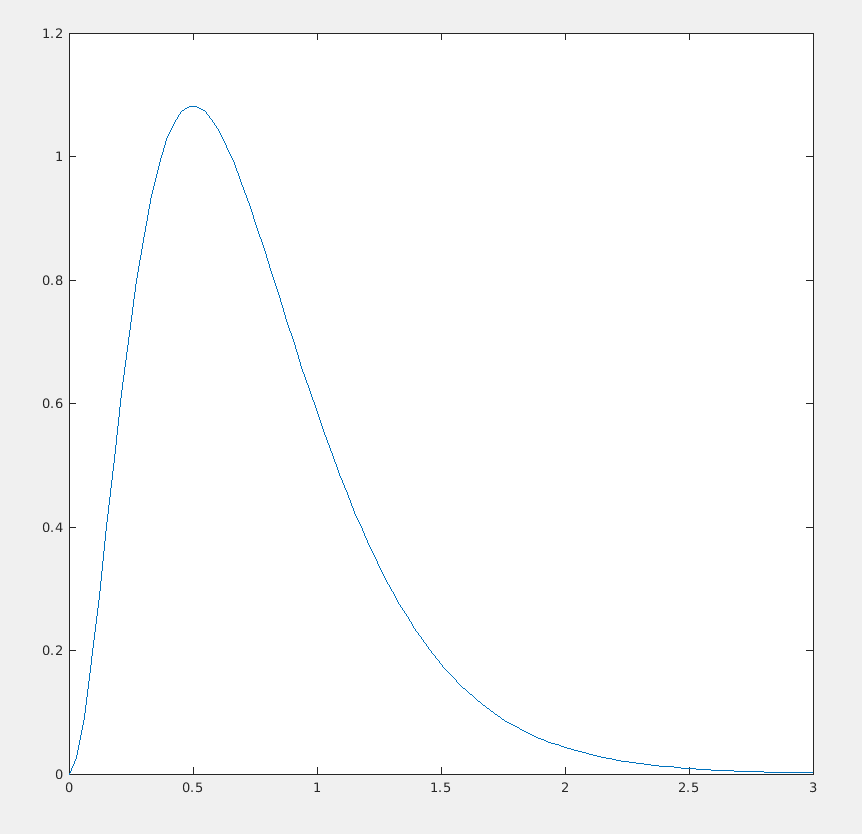
\includegraphics[width=0.5\linewidth]{var8_erlang.png}
	\caption{График закона распределения Эрланга(3,4)}
\end{figure}
 
Для расчета распределения заданной формулы воспользуемся тем, что случайная величина, распределенная по закону Эрланга порядка k и параметром $\lambda$, является суммой k независимых случайных величин, имеющих экспоненциальное распределение с параметром $\lambda$.\\

При этом для экспоненциального закона распределения соотношение выглядит как $a_i = \frac{-1}{\lambda}\ln{R_i}$\\

Таким образом, при k = 3, $\lambda$ = 4 :\\

$a_i^{erl}(k,\lambda) = \sum_{j=1}^3a_j^{exp}(\lambda) = \sum_{j=1}^3\frac{-1}{\lambda}\ln{R_j}$,\\
 \tab \tab \quad \footnotesize{где $R_j$ - равномерное распределение [0,1]}
 
\newpage
 \section*{3. Описание разработанных программ}
 %список использованных переменных, список использованных функций, блок-схема, листинг
 
 \begin{figure}[!h]
	\centering
	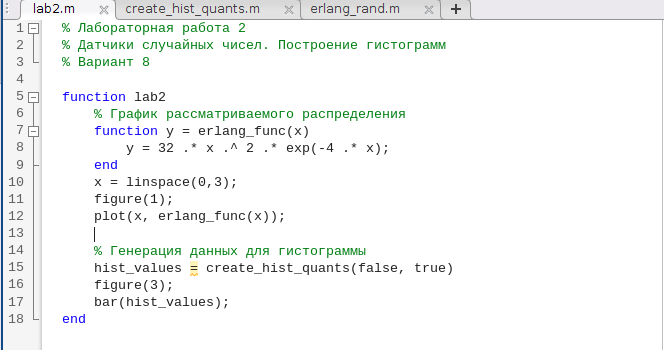
\includegraphics[width=\linewidth]{lab2_code.png}
	\caption{Код main сценария программы}
\end{figure}

Скрипт-сценариий \textbf{\textit{lab2.m}} - точка входа программы, предназначен для запуска всех остальных функции и скриптов, а так же для вывода графиков результатов работы.\\

Основные переменные \textbf{\textit{lab2.m}}:
\begin{itemize}
	\item {\textit{erlang\_func}} - реализация функции плотности вероятности распределения по закону Эрланга при $k = 3, \lambda = 4$
	\item \textit{hist\_values} - посчитанные значения распределения элемнтов сгенерированной выборки по квантам гистограммы
\end{itemize}

\newpage
 
 
\begin{figure}[!h]
	\centering
	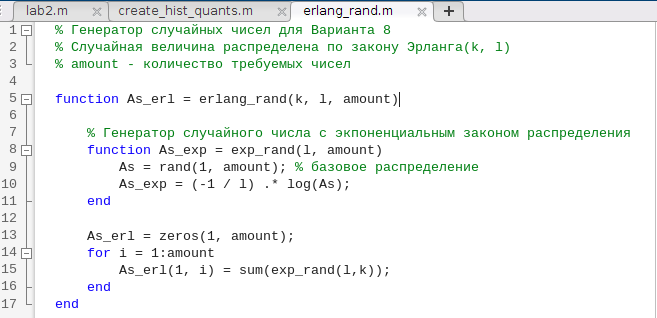
\includegraphics[width=\linewidth]{erlang_rand_code.png}
	\caption{Код для генерации случайных значений}
\end{figure}

Скрипт-функция \textbf{\textit{erlang\_rand.m}} - функция для генерации набора случайных значений по закону Эрланга с параметрами $k = k, l = \lambda$. amount - количество чисел в возвращаемом наборе.\\

Основные переменные \textbf{\textit{erlang\_rand.m}}:
\begin{itemize}
	\item {\textit{exp\_rand}} - реализация генератора случайных чисел с экспоненциальным законом распределения; $l = \lambda$, $amount$ - количество возвращаемых чисел
	\item \textit{As\_erl} - заполняемый набор случайных чисел для распределения по закону Эрланга
\end{itemize}

\newpage

\begin{figure}[!h]
	\centering
	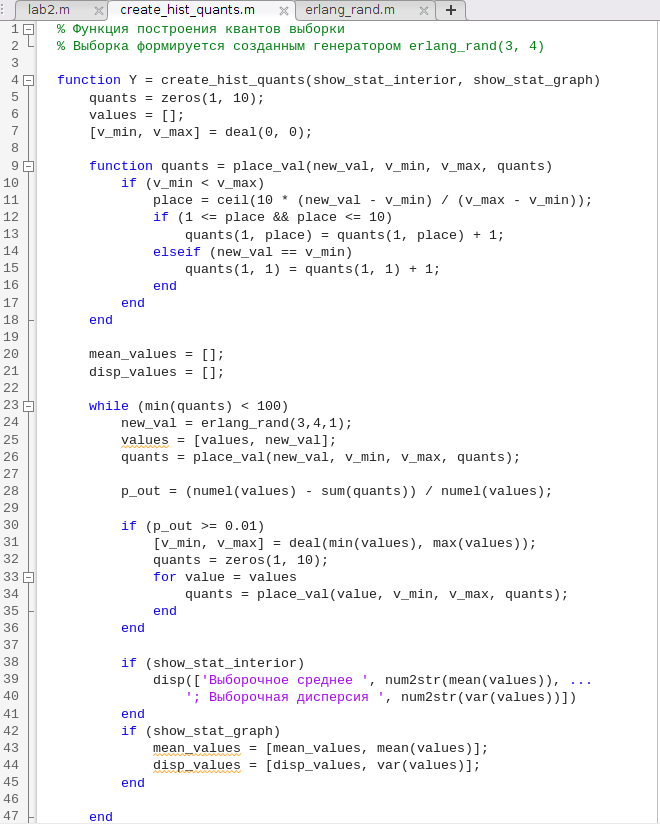
\includegraphics[width=1.04\linewidth]{hists_code_1.png}
	\caption{Код построения квантов: генерация случайных величин}
\end{figure}

 \begin{figure}[!h]
	\centering
	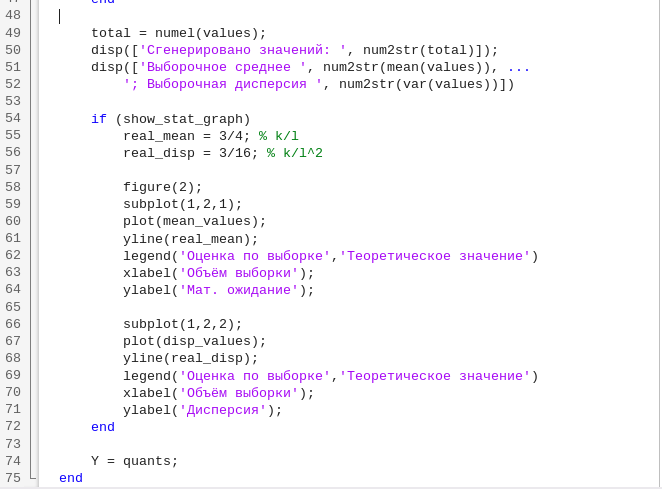
\includegraphics[width=\linewidth]{hists_code_2.png}
	\caption{Код построения квантов: ститистические оценки}
\end{figure}

Скрипт-функция \textbf{\textit{create\_hist\_quants.m}} - функция построения квантов для гистограммы выборки, сформированной генератором \textbf{\textit{erlang\_rand}}. Функция автоматически подбирает конфигурацию подинтервалов и объём выборки.\\

Входные boolean флаги \textit{show\_stat\_*} позволяют выводить информацию о статистических данных во время построения квантов:
\begin{description}
	\item [show\_stat\_interior] даёт возможность на каждом цикле выводить оценки математического ожидания и дисперсии по выборке
	\item [show\_stat\_graph] строит график зависимости оценок математического ожидания и дисперсии от объема выборки\\
\end{description}

Основные переменные \textbf{\textit{create\_hist\_quants.m}}:
\begin{itemize}
	\item \textit{quants} - возвращаемый набор квантов
	\item \textit{values} - значения выборки, генерируемой функцией \textbf{\textit{erlang\_rand}}
	\item \textit{v\_min, v\_max} - минимальное и максимальное значения при построении гистограммы для выборки
	\item \textit{place\_val} - функция, которая "кладёт" значение \textit{new\_val} в правильный квант массива \textit{quants}
	\item \textit{mean\_values, disp\_values} - массивы для запоминания оценок мат.ожидания и дисперсии во время работы алгоритма; имеют смысл только при \textit{show\_stat\_graph} = true
	\item \textit{real\_mean, real\_disp} - аналитически посчитанные значения мат.ожидания, дисперсии для случайных чисел генератора \textbf{\textit{erlang\_rand}}; имеют смысл только при \textit{show\_stat\_graph} = true\\
\end{itemize}

Перерасчёт значений \textit{v\_min, v\_max} происходит не при каждом новом элементе в выборке, а только тогда, когда доля значений выборки за пределами интервала гистограммы $\geq 0.01$. Это позволяет добиться большей выразительности конечной гистограммы.

Для обеспечения приемлемой точности моделирования принято считать, что каждое событие в процессе должно происходить не менее 100 раз. Таким образом, условием остановки генерации новых элементов выборки является то, что каждое значение массива \textit{quants} должно быть не меньше 100.

\newpage
 \section*{4. Представление результатов анализа выборки}
 
 \begin{figure}[!h]
	\centering
	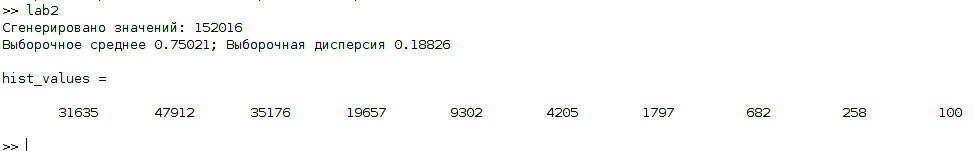
\includegraphics[width=\linewidth]{hist_values_example.png}
	\caption{Пример вывода программы}
\end{figure}

Заполним данными таблицу распределения элементов выборки по квантам гистограммы

\begin{center}
	\begin{tabular}[c]{l|cccccccccc}
  		Номер интервала & 1 & 2 & 3 & 4 & 5 & 6 & 7 & 8 & 9 & 10 \\\hline
  		&&&\\
		Число элементов & 31635 & 41912 & 35176 & 19657 & 9302 & 4205 & 1797 & 682 & 258 & 100\\
	\end{tabular}
\end{center}
 
 \section*{5. Гистограмма сформированной выборки}
 
\begin{figure}[!h]
	\centering
	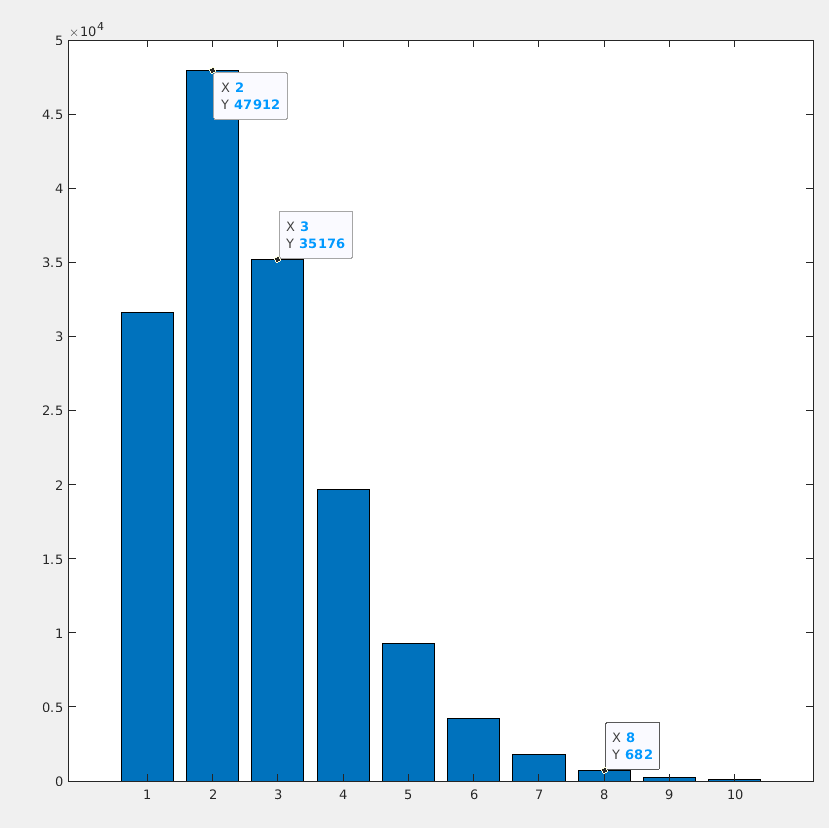
\includegraphics[width=0.5\linewidth]{hist_example.png}
	\caption{Гистограмма для полученной выборки}
\end{figure}
Полученная гистограмма соответсвует исходному графику закона распределения по Эрлангу

\newpage
 \section*{6. Графики зависимости оценок мат. ожидания и дисперсии от объема выборки}
 %На графиках уровнем отметить теоретические значения этиx величин
 
%\begin{figure}[!h]
%	\centering
%	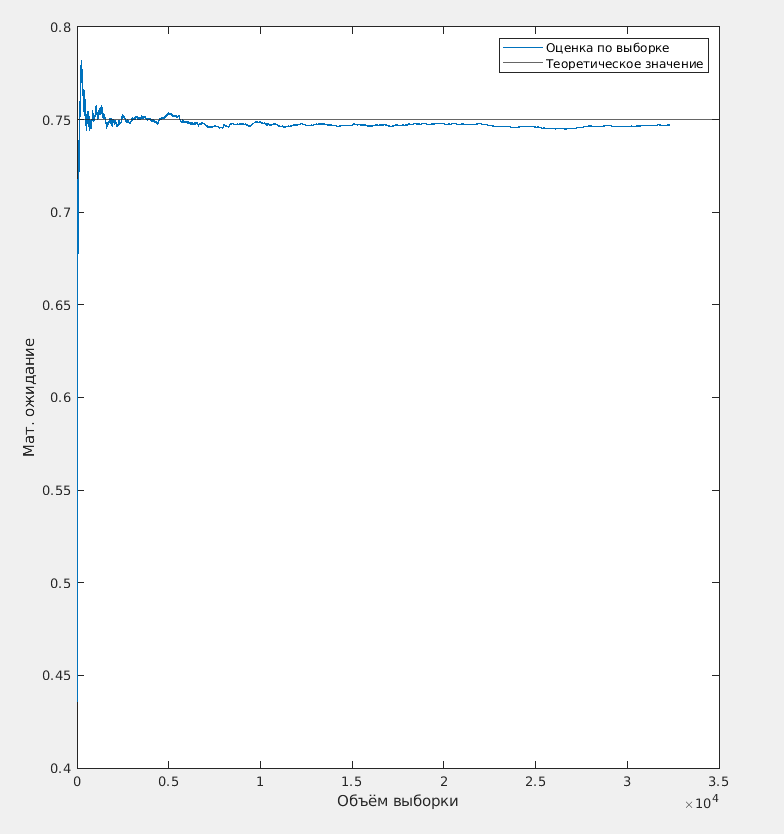
\includegraphics[width=0.5\linewidth]{mean_graph.png}
%	\caption{Сравнение значений математического ожидания выборки}
%\end{figure}

Для распределения по закону Эрланга(k,$\lambda$) существуют аналитическое выражение для математического ожидания и дисперсии:\\

$ Mean = \frac{k}{\lambda}$\\

$ Variance = \frac{k}{\lambda^2}$\\

Получается, при k = 3, $\lambda$ = 4:\\
	$Mean = 0.75; Variance = 0.1875$ \\
	
Сравним эти значения с выборочными средним $\overline X$ и дисперсией $S^2$ в процессе генерации выборки

\begin{figure}[!h]
	\centering
	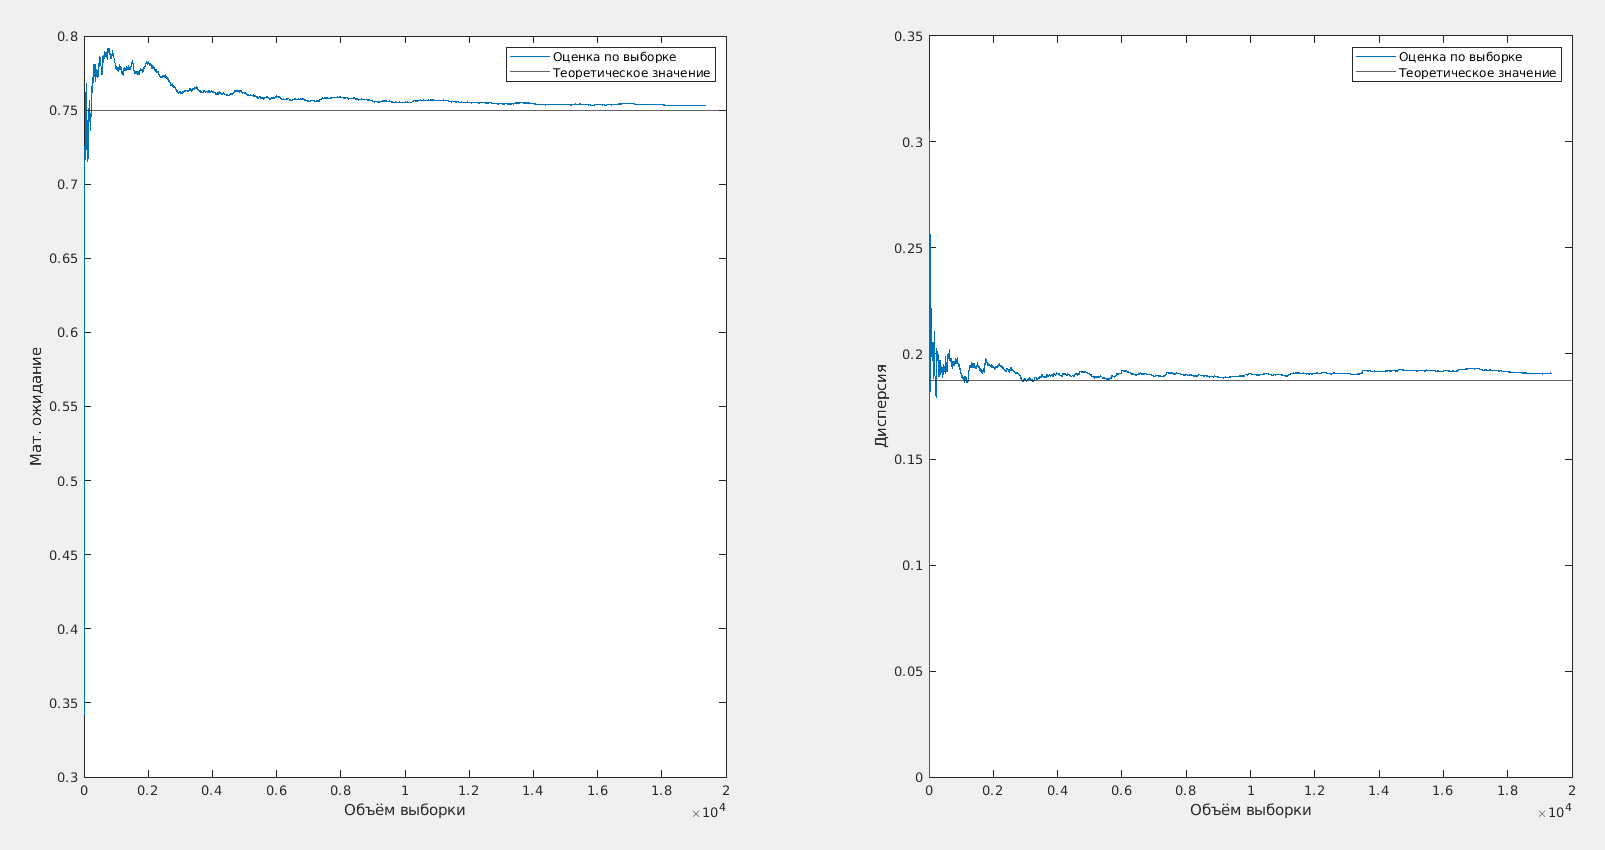
\includegraphics[width=\linewidth]{mean_disp_graph.png}
	\caption{Сравнение статистических значений выборки}
\end{figure}

Видно, что при увеличении N - объема выборки - значения $\overline X$ и $S^2$ стремятся к своим теоретическим значениям.


\newpage
 \section*{7. Выводы}
Целью данной лабораторной работы было изучение алгоритмов получения на ЭВМ чисел с заданным законом распределения и построения гистограмм.\\

В процессе выполнения был реализован способ генерации случайных чисел с эрланговским законом распределения.\\

Для выборок, полученных данным генератором были построены гистограмма и графики зависимости значений мат. ожидания и дисперсии от объема выборки.

\end{document}